\section{Implementation Details}
\label{supp:implementation-details}

We use the \href{https://github.com/PKU-Alignment/safe-rlhf}{Safe-RLHF repository} \citep{dai2023safe} and build RAD on top of their publicly available codebase. For our Safe-RLHF runs, we use the hyperparameters 
reported in their paper. For our RAD implementation, we use REINFORCE \citep{williams1992simple} with the RLOO variance-reduction baseline \citep{Kool2019Buy4R} and $k=2$ samples per prompt. To compute the quantiles required for the RAD policy gradient, we gather samples 
across all GPUs before computing quantiles, increasing the number of available samples. The particle gradient is computed using the Python Optimal Transport library \citep{flamary2021pot}. All RAD models were 
trained on two NVIDIA A100 GPUs, while Safe-RLHF runs required four NVIDIA A100 GPUs due to the additional memory overhead of storing and training the critic network.

\begin{table}[h]
\centering
\begin{tabular}{lc}
\toprule
Hyperparameter & Value \\
\midrule
Sinkhorn regularization $\chi$ & $0.01$ \\
KL coefficient $\beta$ (same value used for Safe RLHF) & $0.1$ \\
$\kappa$ & $10$ \\
Spectral-Wang $\lambda$ & $0.7$ \\
Spectral-Exponential $\lambda$  & $3.0$ \\
Spectral-Power $\lambda$ & $2.0$ \\
Gaussian bandwidth (for VaR) & $0.1$ \\
$\alpha$ ($\textrm{CVaR}_{\alpha}$ / $\textrm{VaR}_{\alpha}$) & $0.9$ \\
\bottomrule
\end{tabular}
\caption{RAD-specific hyperparameters. All other hyperparameters are the same as ones used in Safe-RLHF, unless specified otherwise.}
\label{tab:hyperparams}
\end{table}

\section{RLHF}
\label{supp:RLHF}

%%%%%%%%%%%%%%%%%%%%%%%%%%%%%%%%%%%%%%
Reinforcement Learning from Human Feedback (RLHF) \citep{Christiano2017DeepRL,Ouyang2022TrainingLM} is currently the predominant strategy for aligning Large Language Models (LLMs) with human intent and preferences. The process typically begins with a pre-trained base model, which has been trained on internet-scale data via a next-token prediction objective. The standard RLHF pipeline generally consists of three distinct stages: Supervised Fine-Tuning (SFT), Reward Modeling (RM), and Reinforcement Learning (RL). We detail each of these stages below.

\paragraph{Supervised Fine-Tuning} In the SFT stage, the pre-trained model is trained to follow instructions, via a next-token prediction objective. This process utlizes a high quality dataset of prompt-responses pairs $D_\mathrm{sft}$, where the responses are provided by either a human or LLM annotator \citep{Bai2022ConstitutionalAH}. We refer to the resulting policy from the SFT stage as $\pi_\mathrm{sft}$.

\paragraph{Reward Modeling.}
In the reward modeling stage, we train a reward model to capture human preferences. This stage relies on a dataset of human preferences $D_{\mathrm{pref}} = \{(x_i, y_i^+, y_i^-)\}_{i=1}^N$, where $x_i$ is a prompt, $y_i^+$ is the preferred response to $x_i$, and $y_i^-$ is the dispreferred response to $x_i$. Preference annotations are collected either from human annotators or LLM annotators. Preferences are modeled using the Bradley--Terry preference model \citep{bradley1952rank}, where the log-odds of an observed preference equals the difference between the rewards assigned to the preferred and dispreferred responses by a latent reward function $r(x,y)$:
\begin{equation}
  P(y^+ \succ y^- \mid x)
  =
  \frac{e^{r(x,y^+)}}{e^{r(x,y^+)} + e^{r(x,y^-)}}
  =
  \sigma\big(r(x,y^+) - r(x,y^-)\big),
\end{equation}
where $\sigma$ denotes the sigmoid function. A parameterized reward function with parameters $\phi$ is learned to approximate the latent reward function through maximum likelihood estimation on the preference dataset $D_{\mathrm{pref}}$, using the following objective:
\begin{equation}
  \min_{\phi}
  -\mathbb{E}_{(x,y^{+},y^{-}) \sim D_\mathrm{pref}}
  \big[
    \log \sigma\big(r_{\phi}(x,y^+) - r_{\phi}(x,y^-)\big)
  \big].
  \label{eq:bt_rm_loss}
\end{equation}

\paragraph{Reinforcement Learning} In the Reinforcement Learning stage, a language model or policy is trained to generate responses that are preferred by humans by maximizing the reward of generated responses, as measured by the reward model $r_{\phi}(x,y)$. However, directly optimizing the reward of model generations can lead to degradation in response quality \citep{stiennon2022learningsummarizehumanfeedback,Ouyang2022TrainingLM, Jaques2019WayOB} due to a phenomenon known as reward overoptimization \citep{Gao2022ScalingLF,Rafailov2024ScalingLF}, where the model overfits to imperfections in the learned proxy reward function. To mitigate this effect, a KL penalty term is added to the objective to penalize the model (policy) from drifting too far away from a reference policy, usually chosen to be $\pi_{\mathrm{sft}}$. The RL objective can be expressed as

\begin{equation}
  \max_{\theta} \mathbb{E}_{x \sim \mathcal{D}_x, y \sim \pi_{\theta}(.\vert x)} [r_{\phi}(x,y)] - \beta \mathbb{D}_\mathrm{KL}\big(\pi_{\theta}(.\vert x) \vert\vert \pi_\mathrm{ref}(. \vert x)\big)
\end{equation}

Denoting the KL-regularized reward as $\Tilde{r}(x,y) = r_{\phi}(x,y)-\beta \log \frac{\pi_{\theta}(y \vert x)}{\pi_\mathrm{ref}(y \vert x)}$, we can express the RL objective compactly as

\begin{equation}
  \max_{\theta} \mathbb{E}_{x \sim \mathcal{D}_x, y \sim \pi_{\theta}(.\vert x)}[\Tilde{r}(x,y)]
\end{equation}

The RL objective can be optimized using a variety of reinforcement learning algorithms, such as Proximal Policy Optimization (PPO) \citep{schulman2017proximalpolicyoptimizationalgorithms}, Group Relative Policy Optimization (GRPO) \citep{shao2024deepseekmathpushinglimitsmathematical}, or REINFORCE \citep{williams1992simple,ahmadian2024basicsrevisitingreinforcestyle}.

\section{Entropic Regularization of Optimal Tranport and the Sinkhorn Algorithm}
\label{supp:ot}

% Optimal Transport \citep{peyre2020computationaloptimaltransport} studies the problem of optimally transforming a distribution $\mu$ into another distribution $\nu$ under a cost function
% $c(x,y) : \mathcal{X} \times \mathcal{Y} \to \mathbb{R}_+$, which represents the cost of moving a unit mass from $x$ to $y$.

% Let $\mu$ and $\nu$ be two empirical (atomic) distributions on $\mathbb{R}^{d}$:
% \begin{equation}
%   \mu = \sum_{i=1}^N a_i\,\delta_{x_i}, \qquad \nu = \sum_{j=1}^M b_j\,\delta_{y_j},
%   \label{eq:empirical-dists}
% \end{equation}
% where $x_i, y_j \in \mathbb{R}^d$ are support points (“particles”), $a \in \Delta^N$ and $b \in \Delta^M$ are nonnegative weights summing to 1 ($\Delta^N$ denotes the $N$-dimensional probability simplex), and $\delta_z$ is a Dirac mass at $z$.

% A \emph{transport plan} (a.k.a. coupling) from $\mu$ to $\nu$ is a nonnegative matrix $P \in \mathbb{R}_+^{N \times M}$ whose row and column sums match the marginals. Intuitively, $P_{ij}$ represents the amount of probability mass moved from $x_i$ to $y_j$. The set of admissible couplings can be represented as:
% \begin{equation}
%   \Pi(a,b) := \Bigl\{ P \in \mathbb{R}_+^{N \times M} \;:\; P \mathbf{1}_M = a, \;\; P^\top \mathbf{1}_N = b \Bigr\}.
%   \label{eq:transport-plans}
% \end{equation}

% Given a ground cost function $c:\mathbb{R}^d \times \mathbb{R}^d \to \mathbb{R}_+$, define the cost matrix $C_{ij} = c(x_i, y_j)$. The \textbf{Kantorovich optimal transport problem} \citep{peyre2020computationaloptimaltransport} between $\mu$ and $\nu$ is
% \begin{equation}
%   \mathrm{OT}_c(\mu, \nu) := \min_{P \in \Pi(a,b)} \langle P, C \rangle
%   = \min_{P \in \Pi(a,b)} \sum_{i=1}^N \sum_{j=1}^M P_{ij}\, c(x_i, y_j).
%   \label{eq:kantorovich-ot-supp}
% \end{equation}

% A common choice for the cost function is the $p$-norm of the difference between points:
% \begin{equation}
%   c(x_i, y_j) = \| x_i - y_j \|_p^p, \quad p \ge 1,
% \end{equation}
% which leads to the definition of the \emph{$p$-Wasserstein distance} between $\mu$ and $\nu$, denoted as $\mathcal{W}_{p}(\mu, \nu)$.
% \begin{equation}
%   \mathcal{W}_p(\mu, \nu) := \Big(\min_{P \in \Pi(a,b)} \sum_{i=1}^N \sum_{j=1}^M P_{ij}\, \|x_i - y_j\|_p^p.\Big)^{\frac{1}{p}}
%   \label{eq:wasserstein-distance}
% \end{equation}

% \subsection{Entropic Regularization and the Sinkhorn Algorithm}

The unregularized optimal transport problem in \Cref{eq:kantorovich-ot} can be solved using linear programming \citep{dantzig2016linear, dvurechensky2018computational}, but this can be computationally expensive when the number of particles is large. Hence, an entropy regularization term is typically added to the objective,
% Hence, we use entropic regularization, which adds an entropy term to the objective and
which allows for efficient optimization using the Sinkhorn algorithm \citep{cuturi2013sinkhorn}. Specifically, we define the entropic regularized OT problem between distributions $\mu$ and $\nu$ as:
\begin{equation}
  \mathrm{OT}_{c}^\chi(\mu,\nu) \;=\; \min_{P\in\Pi(\mu,\nu)}\;\langle P,C\rangle - \chi H(P), \quad H(P)\;=\;-\sum_{i,j} P_{ij}\log P_{ij},
  \label{eq:entropic-ot}
\end{equation}
for a regularization parameter $\chi>0$ and a cost matrix $C$. Recall that $\Pi(\mu,\nu)$ represents the set of admissible couplings as stated in~\eqref{eq:transport-plans} (and defined by the marginal of $\mu$ and $\nu$). This problem is strictly convex in  $P$  and has a unique minimizer  $P^\star$. More importantly, it can be solved efficiently using the Sinkhorn algorithm \citep{cuturi2013sinkhorn}, which iteratively updates scaling vectors to enforce the marginal constraints. The resulting transport plan  $P^\star$  can then be used to compute the optimal transport objective and its gradient with respect to the policy parameters  $\theta$. We now decribe how to compute the optimal transport objective.

Let the marginals of $\mu$ and $\nu$ be the vectors $a$ and $b$ respectively. Define the Gibbs kernel
\begin{equation}K_{ij} \;=\; e^{-C_{ij}/\chi}.
  \label{eq:gibbs-kernel}
\end{equation}The optimal transport plan can be expressed in closed form as
\begin{equation}P^\star \;=\; \mathrm{diag}(u) K \mathrm{diag}(v),
  \label{eq:optimal-plan}
\end{equation}where  $u \in \mathbb{R}^N$, $v\in\mathbb{R}^M$  are scaling vectors that can be computed using the Sinkhorn iterations
\begin{equation}u^{(t+1)} \;=\; \frac{a}{Kv^{(t)}}, \qquad v^{(t+1)} \;=\; \frac{b}{K^\top u^{(t+1)}},
  \label{eq:sinkhorn-iterations}
\end{equation}starting from some positive initialization (e.g.  $u^{(0)}=v^{(0)}=\mathbf 1$). The iterations are guaranteed to converge to the unique optimal plan  $P^\star$  that satisfies the marginal constraints \citep{peyre2020computationaloptimaltransport, cuturi2013sinkhorn}. Once we have  $P^\star$ , we can compute the FSD objective as
\begin{equation}
  \mathcal{L}_{\mathrm{FSD}}^\chi(\mu,\nu) \;=\; \langle P^\star,C\rangle - \chi H(P^\star).
  \label{eq:fsd-loss-sinkhorn}
\end{equation}

Because the algorithm consists only of a fixed number of matrix-vector multiplications and divisions, gradients can be propagated through the iterations using automatic differentiation in frameworks like PyTorch \citep{NEURIPS2019_9015} or JAX \citep{jax2018github}, making the Sinkhorn algorithm end to end differentiable.

\section{FSD}
\label{supp:FSD}

\begin{theorem}[from \citet{melnyk2024distributional}]
  \label{thm:fsd_as_ot}
  Let $h : \mathbb{R} \to \mathbb{R}_{+}$ be a convex function, and let
  $X$ and $Y$ be real-valued random variables with probability measures
  $\mu_X$ and $\mu_Y$, respectively. Denote by
  $Q_X, Q_Y : [0,1] \to \mathbb{R}$ their (left-continuous) quantile functions.

  Then,
  \begin{equation}
    \int_0^1 h\big(Q_X(q) - Q_Y(q)\big)\, dq
    =
    \min_{\gamma \in \Pi(\mu_X,\mu_Y)}
    \int_{\mathbb{R}^2} h(x-y)\, d\gamma(x,y),
  \end{equation}
  where $\Pi(\mu_X,\mu_Y)$ denotes the set of all couplings
  (joint probability measures) on $\mathbb{R}^2$ with marginals
  $\mu_X$ and $\mu_Y$. Moreover, if $h$ is strictly convex, the minimizing transport plan $\gamma^\star$ is unique.
\end{theorem}

\begin{corollary}[FSD as asymmetric optimal transport]
  \label{cor:fsd_as_ot}
  Let $X,Y$ be real-valued random variables with measures
  $\mu_X$ and $\mu_Y$, and define the FSD objective
  \[
    \mathcal{L}_{\mathrm{FSD}}(X,Y)
    :=
    \int_0^1 \big(Q_Y(q) - Q_X(q)\big)_+ \, dq.
  \]
  Then
  \[
    \mathcal{L}_{\mathrm{FSD}}(X,Y)
    =
    \min_{\gamma \in \Pi(\mu_X,\mu_Y)}
    \int_{\mathbb{R}^2} (y-x)_+ \, d\gamma(x,y),
  \]
  that is, the FSD objective coincides with the optimal transport cost under the
  asymmetric convex cost function $c(x,y)=(y-x)_+$.
\end{corollary}

\section{Derivation of Theorem~\ref{thm:sard_pg}}\label{app:sard_pg_derivation}

\subsection{RAD Policy Gradient}
\label{sec:sard-pol-grad}

% Before deriving the policy gradient of the Dual RAD objective in Equation~\ref{eq:sard_dual}, we first fix a representation for the cost distributions appearing in the FSD term. One approach would be to assume a parametric family of distributions and use variational inference to select the member that best approximates the true cost distribution induced by the policy. Alternatively, one may adopt a nonparametric empirical approximation. We take the latter approach.

We represent the cost distribution via a particle approximation in quantile space. Let $\{ q_i \}_{i=1}^{N}$ denote an ordered set of cost quantiles satisfying
\[
  q_1 \leq q_2 \leq \dots \leq q_N .
\]
We approximate the induced cost distribution by the empirical measure
\[
  \hat{\mu} = \frac{1}{N} \sum_{i=1}^{N} \delta_{q_i},
\]
where $\delta_{q_i}$ denotes the Dirac measure located at $q_i$. In practice, this approximation is obtained by sampling generations from the policy, evaluating their associated costs, and computing empirical quantiles from the resulting samples. These quantiles serve as the particles defining the discrete representation of the distribution.

Let $\hat{\mu}_{\pi_{\theta}}$ and $\hat{\mu}_{\pi_{\mathrm{ref}}}$ denote the empirical cost distributions of the policy $\pi_{\theta}$ and $\pi_{\mathrm{ref}}$ respectively. Note that we represent $C_{\pi_{\theta}}$ and $C_{\pi_{\mathrm{ref}}}$ using their quantiles $\{q_{i}(\pi_{\theta})\}_{i=1}^{N}$ and $\{q_{i}(\pi_{\mathrm{ref}})\}_{i=1}^{N}$ respectively. The gradient of the FSD objective can be expressed using the chain rule as follows.
\begin{align}
  \nabla_{\theta} \mathcal{L}_{\mathrm{FSD}}\!\big(\hat{\mu}_{\pi_{\theta}},\,\hat{\mu}_{\pi_{\mathrm{ref}}}\big) &= \nabla_{\theta} \mathcal{L}_{\mathrm{FSD}}\big(\{q_{i}(\pi_{\theta})\}_{i=1}^{N}, \{q_{i}(\pi_{\mathrm{ref}})\}_{i=1}^{N}\big)\\
  %
  &= \sum_{i=1}^{N} \frac{\partial \mathcal{L}_{\mathrm{FSD}}}{\partial q_i(\pi_{\theta})} \frac{\partial q_i(\pi_{\theta})}{\partial \theta} = \Big\langle \nabla_{q(\pi_{\theta})}\mathcal{L}_{\mathrm{FSD}}, \nabla_{\theta} q(\pi_{\theta}) \Big\rangle
\end{align}

We denote the gradient vector $\nabla_{q(\pi_{\theta})}\mathcal{L}_{\mathrm{FSD}}$ as the particle gradient. This gradient vector tells us how the FSD objective changes when the particles (quantiles in our setting) used to approximate the empirical distribution of costs of the policy generations are perturbed slightly. The other gradient vector $\nabla_{\theta} q(\pi_{\theta})$ is the quantile gradient, which tells us how the quantiles of the cost distribution change, when the policy parameters are perturbed slightly.

\paragraph{Estimating the Particle Gradient} The FSD objective can be reinterpreted as an optimal transport problem with an asymmetric cost
$c(x,y) = (y - x)_{+}$ as decribed in Corollary~\ref{cor:fsd_as_ot}. The particle gradient can then be viewed as the sensitivity of the optimal transport objective to infinitesimal perturbations of the particle locations.

The classical optimal transport problem (as described in~\eqref{eq:kantorovich-ot}) between $\hat{\mu}_{\pi_\theta}$ and $\hat{\mu}_{\pi_{\mathrm{ref}}}$ is
\begin{equation}
  \mathrm{OT}_c(\hat{\mu}_{\pi_{\theta}},\,\hat{\mu}_{\pi_{\mathrm{ref}}}) := \min_{P \in \Pi(\hat{\mu}_{\pi_{\theta}},\,\hat{\mu}_{\pi_{\mathrm{ref}}})} \langle P, C \rangle
  = \min_{P \in \Pi(\hat{\mu}_{\pi_{\theta}},\,\hat{\mu}_{\pi_{\mathrm{ref}}})} \sum_{i=1}^N \sum_{j=1}^M P_{ij}\, c(x_i, y_j).
  \label{eq:kantorovich-ot-supp}
\end{equation}
where $C_{ij} = c(x_i, y_j)$ is the the cost matrix. Recall that $\Pi(\hat{\mu}_{\pi_{\theta}},\,\hat{\mu}_{\pi_{\mathrm{ref}}}) $ is the set of admissible couplings defined as $\Pi(\hat{\mu}_{\pi_{\theta}},\,\hat{\mu}_{\pi_{\mathrm{ref}}}) := \Bigl\{ P \in \mathbb{R}_+^{N \times N} \;:\; P \mathbf{1}_M = a, \;\; P^\top \mathbf{1}_N = b \Bigr\}.$ The vectors $a$ and $b$ represent the marginals. In our case, the marginals of the empirical cost distributions are $\frac{1}{N}$. 

The classical optimal transport objective as described in~\eqref{eq:kantorovich-ot-supp} is not smooth with respect to particle positions. It is also non-differentiable and small perturbations in particle locations can induce discontinuous changes in the optimal coupling $P^*$. To address these issues, we instead consider the entropy-regularized optimal transport problem as described in~\eqref{eq:entropic-ot}. The regularized objective
\[
  \mathcal{L}_{\mathrm{FSD}}^{\chi}(\hat{\mu}_{\pi_{\theta}},\,\hat{\mu}_{\pi_{\mathrm{ref}}})
  =
  OT^{\chi}_{(y-x)_{+}}\!\left(\hat{\mu}_{\pi_{\theta}},\,\hat{\mu}_{\pi_{\mathrm{ref}}}\right)
\]
adds a strictly convex entropic penalty to the transport plan, yielding a smooth objective that is differentiable with respect to the particle positions. The solution can be computed efficiently using the Sinkhorn algorithm, enabling end-to-end differentiation as described in Section~\ref{supp:ot}.

The regularized objective $\mathcal{L}_{\mathrm{FSD}}^{\chi}$ is a smooth approximation of the original FSD objective $\mathcal{L}_{\mathrm{FSD}}$.
\[
  \mathcal{L}_{\mathrm{FSD}}^{\chi}
  \;\longrightarrow\;
  \mathcal{L}_{\mathrm{FSD}}
  \quad \text{as } \chi \to 0.
\]
In practice, $\chi$ is chosen to balance approximation bias and numerical stability.

\paragraph{Estimating the Quantile Gradient} The quantile gradient informs us how all the quantiles in our empirical distribution of costs of policy generations, change when the policy parameters are perturbed slightly. We consider only the quantile gradient of a single quantile here. The quantile gradient wrt all quantiles can be computed in a similiar manner. Let $F_{\theta}$ be the cumulative distribution function (CDF) of the cost distribution of the model outputs under policy $\pi_{\theta}$. The quantile gradient of a particular quantile $q_i$ is canonically given by $$\nabla_\theta q_i(\pi_\theta)= -\frac{\nabla_\theta F_\theta(t)\vert_{t=q_i}}{f_\theta(q_i)}.$$ Since the PDF in the denominator is unknown, the derivative can be approximated as \citep{li2024tiltedquantilegradientupdates}
\begin{equation}
  \nabla_{\theta} q_{i}(\pi_{\theta}) \approx -\nabla_{\theta} F_{\theta}(q) \Big\vert_{q = q_{i}(\pi_{\theta})}
\end{equation}

The CDF $F_{\theta}$ can be expressed as an expectation and we can use the REINFORCE trick \citep{williams1992simple} to compute the policy gradient of the CDF of the cost distribution of model generations.
\begin{align}
  \nabla_{\theta} F_{\theta}(q) &= \nabla_{\theta} \mathbb{E}_{x \sim \mathcal{D}_{x}, y \sim \pi_{\theta}(. \vert x)} \Big[ \mathds{1}(c_{\psi}(x,y) \leq q)\Big] \\
  &= \mathbb{E}_{x \sim \mathcal{D}_{x}, y \sim \pi_{\theta}(. \vert x)} \Big[ \mathds{1}(c_{\psi}(x,y) \leq q) \nabla_{\theta} \log \pi_{\theta}(y \vert x)\Big]
\end{align}
Recall that the cost distribution is defined via the learned cost model $c_{\psi}(x,y)$ where $x \sim \mathcal{D}_{x}$ is the input prompt and $y \sim \pi_{\theta}(. \vert x)$ is the model output. The quantile gradient for $q_i$ can then be expressed as
\begin{equation}
  \nabla_{\theta} q_{i}(\pi_{\theta}) \approx -\mathbb{E}_{x \sim \mathcal{D}_{x}, y \sim \pi_{\theta}(. \vert x)} \Big[ \mathds{1}(c_{\psi}(x,y) \leq q_i) \nabla_{\theta} \log \pi_{\theta}(y \vert x)\Big]
  \label{eq:quantile-gradient}
\end{equation}

\paragraph{Putting it all together} Using the particle gradient and the quantile gradient, the gradient of the FSD objective with respect to policy parameters can be expressed as

\begin{align}
  \nabla_{\theta} \mathcal{L}_{\mathrm{FSD}}(\hat{\mu}_{\theta}, \hat{\mu}_{\mathrm{ref}}) &= \sum_{i=1}^{N} \frac{\partial \mathcal{L}^{\chi}_{\mathrm{FSD}}}{\partial q_i(\pi_{\theta})} \frac{\partial q_i(\pi_{\theta})}{\partial \theta} \\
  &= \sum_{i=1}^{N} -\frac{\partial \mathcal{L}^{\chi}_{\mathrm{FSD}}}{\partial q_i(\pi_{\theta})} \mathbb{E}_{x \sim \mathcal{D}_{x}, y \sim \pi_{\theta}(. \vert x)} \Big[ \mathds{1}(c_{\psi}(x,y) \leq q_i) \nabla_{\theta} \log \pi_{\theta}(y \vert x)\Big]\\
  &=\mathbb{E}_{x \sim \mathcal{D}_{x}, y \sim \pi_{\theta}(. \vert x)}\Big[ \Big(\sum_{i=1}^{N} -\frac{\partial \mathcal{L}^{\chi}_{\mathrm{FSD}}}{\partial q_i(\pi_{\theta})} \mathds{1}(c_{\psi}(x,y) \leq q_i)\Big) \nabla_{\theta} \log \pi_{\theta}(y \vert x)\Big] \label{eq:fsd-gradient}
\end{align}
Denoting the RAD objective as $\max_{\theta} \min_{\lambda \geq 0} \mathcal{L}(\theta, \lambda)$ the RAD policy gradient can then be expressed as
\begin{equation}
  \nabla_{\theta} \mathcal{L}(\theta, \lambda) = \mathbb{E}_{x \sim \mathcal{D}_{x}, y \sim \pi_{\theta}(. \vert x)}\Big[ \Big( \Tilde{r}(x,y) + \lambda \big(\sum_{i=1}^{N} -\frac{\partial \mathcal{L}^{\chi}_{\mathrm{FSD}}}{\partial q_i(\pi_{\theta})} \mathds{1}(c_{\psi}(x,y) \leq q_i)\big)\Big) \nabla_{\theta} \log \pi_{\theta}(y \vert x)\Big]
  \label{eq:sard-policy-gradient}
\end{equation}

We then use REINFORCE \citep{williams1992simple} with RLOO \citep{Kool2019Buy4R} to optimize the RAD objective using the policy gradient expression in Equation ~\ref{eq:sard-policy-gradient}. For the setting, where we weight quantiles differently in the FSD objective as in Equation ~\ref{eq:weighted-fsd-loss-dfn}, the policy gradient can be expressed as follows, only requiring an additional weighting coefficient $w(q_i)$.

\begin{equation}
  \nabla_{\theta} \mathcal{L}(\theta, \lambda) = \mathbb{E}_{x \sim \mathcal{D}_{x}, y \sim \pi_{\theta}(. \vert x)}\Big[ \Big( \Tilde{r}(x,y) + \lambda \big(\sum_{i=1}^{N} -w(q_i) \frac{\partial \mathcal{L}^{\chi}_{\mathrm{FSD}}}{\partial q_i(\pi_{\theta})} \mathds{1}(c_{\psi}(x,y) \leq q_i)\big)\Big) \nabla_{\theta} \log \pi_{\theta}(y \vert x)\Big]
  \label{eq:weighted-sard-policy-gradient}
\end{equation}

%\section{Spectral Risk Measures}


\begin{figure}  % 'r' for right-aligned figure
  \centering
  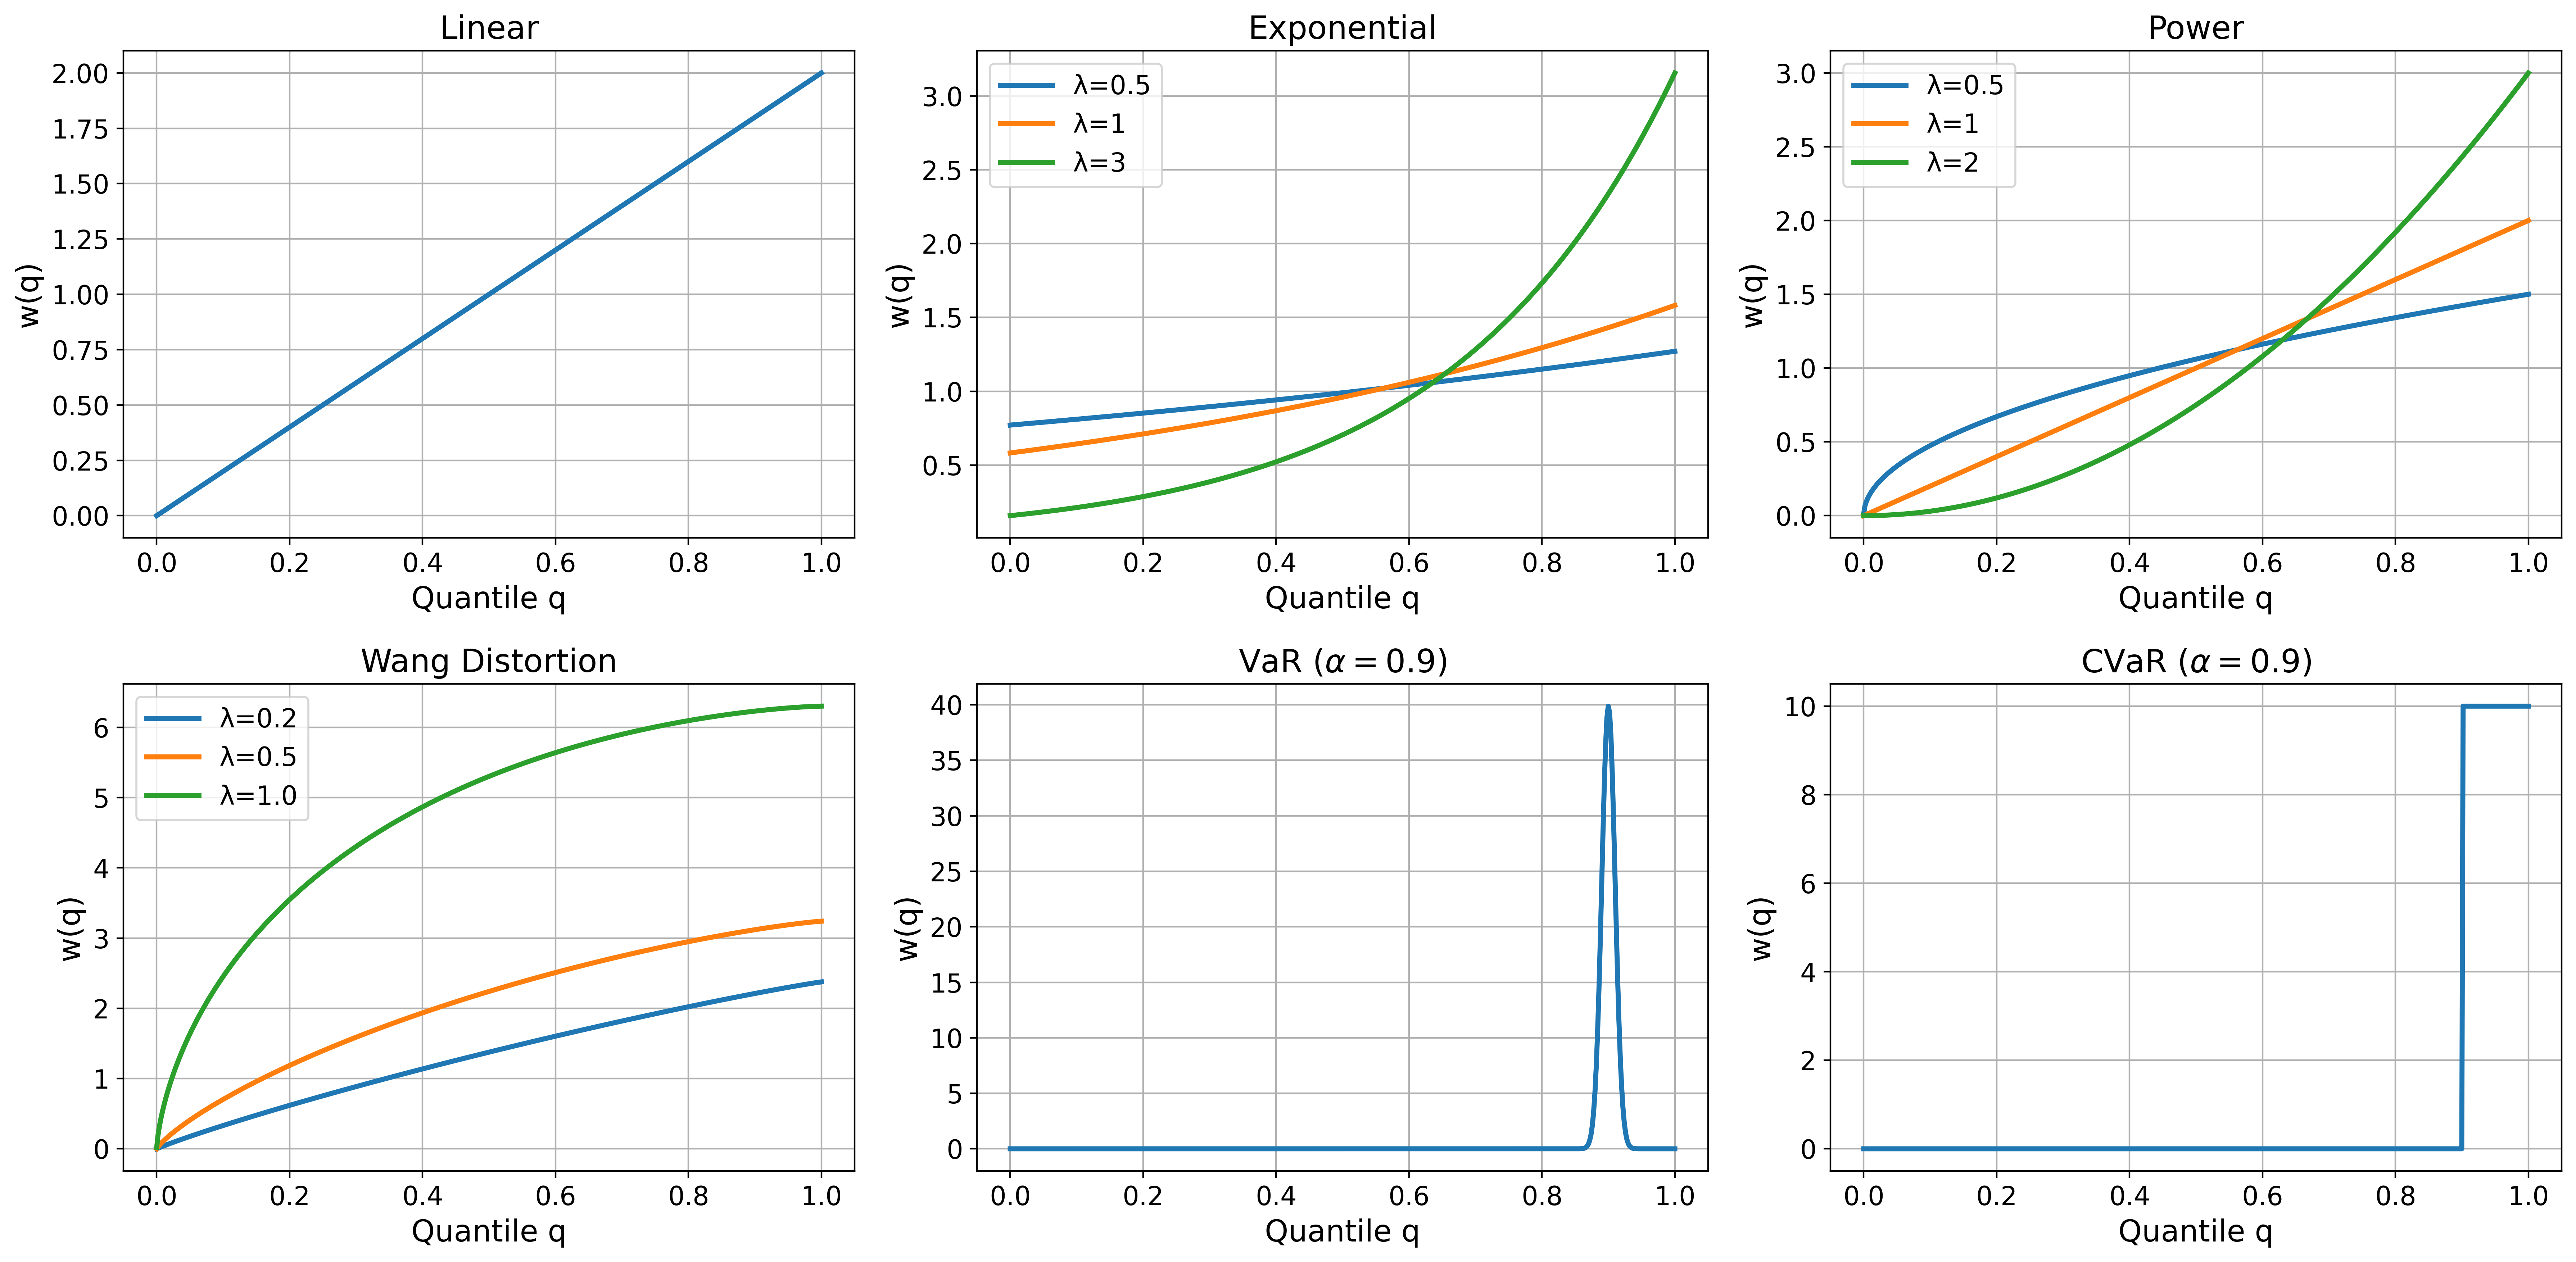
\includegraphics[width=0.9\textwidth]{figs/spectral_weights_comparison.png}
  \caption{Illustration of spectral weighting functions corresponding to different spectral risk measures (SRMs). For parameterized families, the plots show how the spectral weights vary with the risk-aversion parameter $\lambda$. Note that VaR is represented as a gaussian with very small bandwidth instead of a dirac delta for implementation reasons. \yc{add the params used for wang in the plot} } 
  \label{fig:srm-illustration}
\end{figure}

% \aj{-------------------------------}

% This appendix derives the RAD policy-gradient estimator in Theorem~\ref{thm:sard_pg}.
% We decompose the gradient of the FSD term into (i) a \emph{particle gradient} (sensitivity of the FSD loss to quantile-particle locations) and (ii) a \emph{quantile gradient} (sensitivity of those quantile locations to $\theta$), and then combine them.

% \subsection{Quantile-particle approximation of the cost distribution}
% For each policy $\pi$, define the induced cost random variable $C(\pi):=c_\psi(x,y)$ with $x\sim D_x$ and $y\sim\pi(\cdot\mid x)$.
% Fix quantile levels $\alpha_1<\dots<\alpha_N$ in $(0,1)$ and define the corresponding quantile values
% $q_i(\pi):=Q_{C(\pi)}(\alpha_i)$.
% We approximate the cost distribution of $\pi$ by the empirical measure in \emph{quantile-value space}
% \[
%   \hat\mu_\pi \;:=\;\frac1N\sum_{i=1}^N \delta_{q_i(\pi)}.
% \]
% In practice, $q_i(\pi)$ is computed from samples of $C(\pi)$ by empirical quantiles.

% \subsection{Chain-rule decomposition}
% Using the approximation $L_{\mathrm{FSD}}\big(C(\pi_\theta),C(\pi_{\mathrm{ref}})\big)\approx
% L_{\mathrm{FSD}}\big(\hat\mu_{\pi_\theta},\hat\mu_{\pi_{\mathrm{ref}}}\big)$, we write
% \begin{align}
%   \nabla_\theta L_{\mathrm{FSD}}\!\big(\hat\mu_{\pi_\theta},\hat\mu_{\pi_{\mathrm{ref}}}\big)
%   &=
%   \nabla_\theta L_{\mathrm{FSD}}\!\Big(\{q_i(\pi_\theta)\}_{i=1}^N,\{q_i(\pi_{\mathrm{ref}})\}_{i=1}^N\Big) \\
%   &=
%   \sum_{i=1}^N \frac{\partial L_{\mathrm{FSD}}}{\partial q_i(\pi_\theta)}\,\nabla_\theta q_i(\pi_\theta).
% \end{align}
% % which matches the decomposition used in the main draft (Eqs.~(14)--(15)).

% \subsection{Particle gradient via entropic OT and Sinkhorn}
% The unregularized OT formulation of $L_{\mathrm{FSD}}$ with cost $c(x,y)=(y-x)_+$ is generally non-smooth in particle locations.
% We therefore compute particle gradients through the entropically-regularized OT objective
% \[
%   L_{\mathrm{FSD}}^\varepsilon(\hat\mu_{\pi_\theta},\hat\mu_{\pi_{\mathrm{ref}}})
%   :=\mathrm{OT}^{\varepsilon}_{(y-x)_+}(\hat\mu_{\pi_\theta},\hat\mu_{\pi_{\mathrm{ref}}}),
% \]
% whose optimizer admits the Sinkhorn scaling form and is differentiable with respect to particle locations.
% In implementation we run a fixed number of Sinkhorn iterations and backpropagate to obtain
% $\frac{\partial L_{\mathrm{FSD}}}{\partial q_i(\pi_\theta)}$.

% \subsection{Quantile gradient via implicit differentiation and REINFORCE}
% Each quantile value $q_i(\pi_\theta)$ satisfies the defining equation
% \[
%   F_\theta\big(q_i(\pi_\theta)\big)=\alpha_i,
%   \qquad
%   F_\theta(t):=\mathbb{P}\big(C(\pi_\theta)\le t\big).
% \]
% Differentiating w.r.t.\ $\theta$ yields (by the implicit function theorem) the identity
% \[
%   \nabla_\theta q_i(\pi_\theta)
%   =
%   -\frac{\nabla_\theta F_\theta(t)\vert_{t=q_i(\pi_\theta)}}{f_\theta\big(q_i(\pi_\theta)\big)},
% \]
% where $f_\theta$ is the density of $C(\pi_\theta)$ at the quantile (when it exists).
% Estimating $f_\theta$ can be nontrivial; following the main draft, one may absorb $1/f_\theta$ into the step-size or use a density estimate, which leads to the approximation recorded in Eq.~(16) of the draft.

% Next, we express $\nabla_\theta F_\theta(t)$ via the log-derivative trick:
% \begin{align}
%   \nabla_\theta F_\theta(t)
%   &=\nabla_\theta \mathbb{E}_{x\sim D_x,\,y\sim\pi_\theta(\cdot\mid x)}\!\big[\mathbf{1}(c_\psi(x,y)\le t)\big]\\
%   &=
%   \mathbb{E}_{x\sim D_x,\,y\sim\pi_\theta(\cdot\mid x)}\!\big[\mathbf{1}(c_\psi(x,y)\le t)\,\nabla_\theta\log\pi_\theta(y\mid x)\big].
% \end{align}
% Substituting $t=q_i(\pi_\theta)$ and combining with the chain rule gives
% \[
%   \nabla_\theta L_{\mathrm{FSD}}\!\big(\hat\mu_{\pi_\theta},\hat\mu_{\pi_{\mathrm{ref}}}\big)
%   =
%   \mathbb{E}_{x,y}\Bigg[
%     \Bigg(\sum_{i=1}^N
%       \Big(-\frac{\partial L_{\mathrm{FSD}}}{\partial q_i(\pi_\theta)}\Big)\,
%       \mathbf{1}(c_\psi(x,y)\le q_i(\pi_\theta))
%     \Bigg)\nabla_\theta\log\pi_\theta(y\mid x)
%   \Bigg],
% \]
% (up to the density factor discussed above).

% \subsection{Completion of the proof of Theorem~\ref{thm:sard_pg}}
% Finally, since
% $L(\theta,\lambda)=\mathbb{E}[\tilde r(x,y)] + \lambda(L_{\mathrm{FSD}}-\kappa)$,
% adding the standard REINFORCE gradient for $\mathbb{E}[\tilde r(x,y)]$ and grouping terms yields Eq.~\eqref{eq:sard_pg}.
% The weighted case follows identically by inserting weights $w(\alpha_i)$ in the Riemann-sum approximation of $L_{\mathrm{FSD}}^{w}$.
% \qed
